\section{GPDs of Nuclei}

It has been clear for many years that inclusive measurements alone cannot
provide a 
full quantitative explanation of the EMC
effect \cite{Aubert:1983xm}.
Imaging of nuclei, now possible for the first time
through deeply-virtual Compton scattering (DVCS) and deeply-virtual meson production (DVMP), can answer the question using GPDs as a tool \cite{Dupre:2015jha}.
By comparing transverse spatial quark and gluon distributions in nuclei
or bound nucleons (to be obtained in coherent or incoherent DVCS, respectively) to
the corresponding quantities in free nucleons,
one can realize a pictorial representation of the EMC effect.
%Indeed,
%a pictorial representation of the realization of the
%EMC effect will be at hand, through the comparison of 
%quark and gluon distributions 
%in nuclei, in the transverse plane, to be obtained in coherent DVCS, or 
%in bound nucleons, extracted from incoherent DVCS, with the corresponding
%quantities measured for free nucleons.
The presence of non-nucleonic degrees of freedom, 
as addressed in Ref. \cite{primo},
or the 
change of confinement radii in bound nucleons, will be observed. 

\begin{figure}[t]
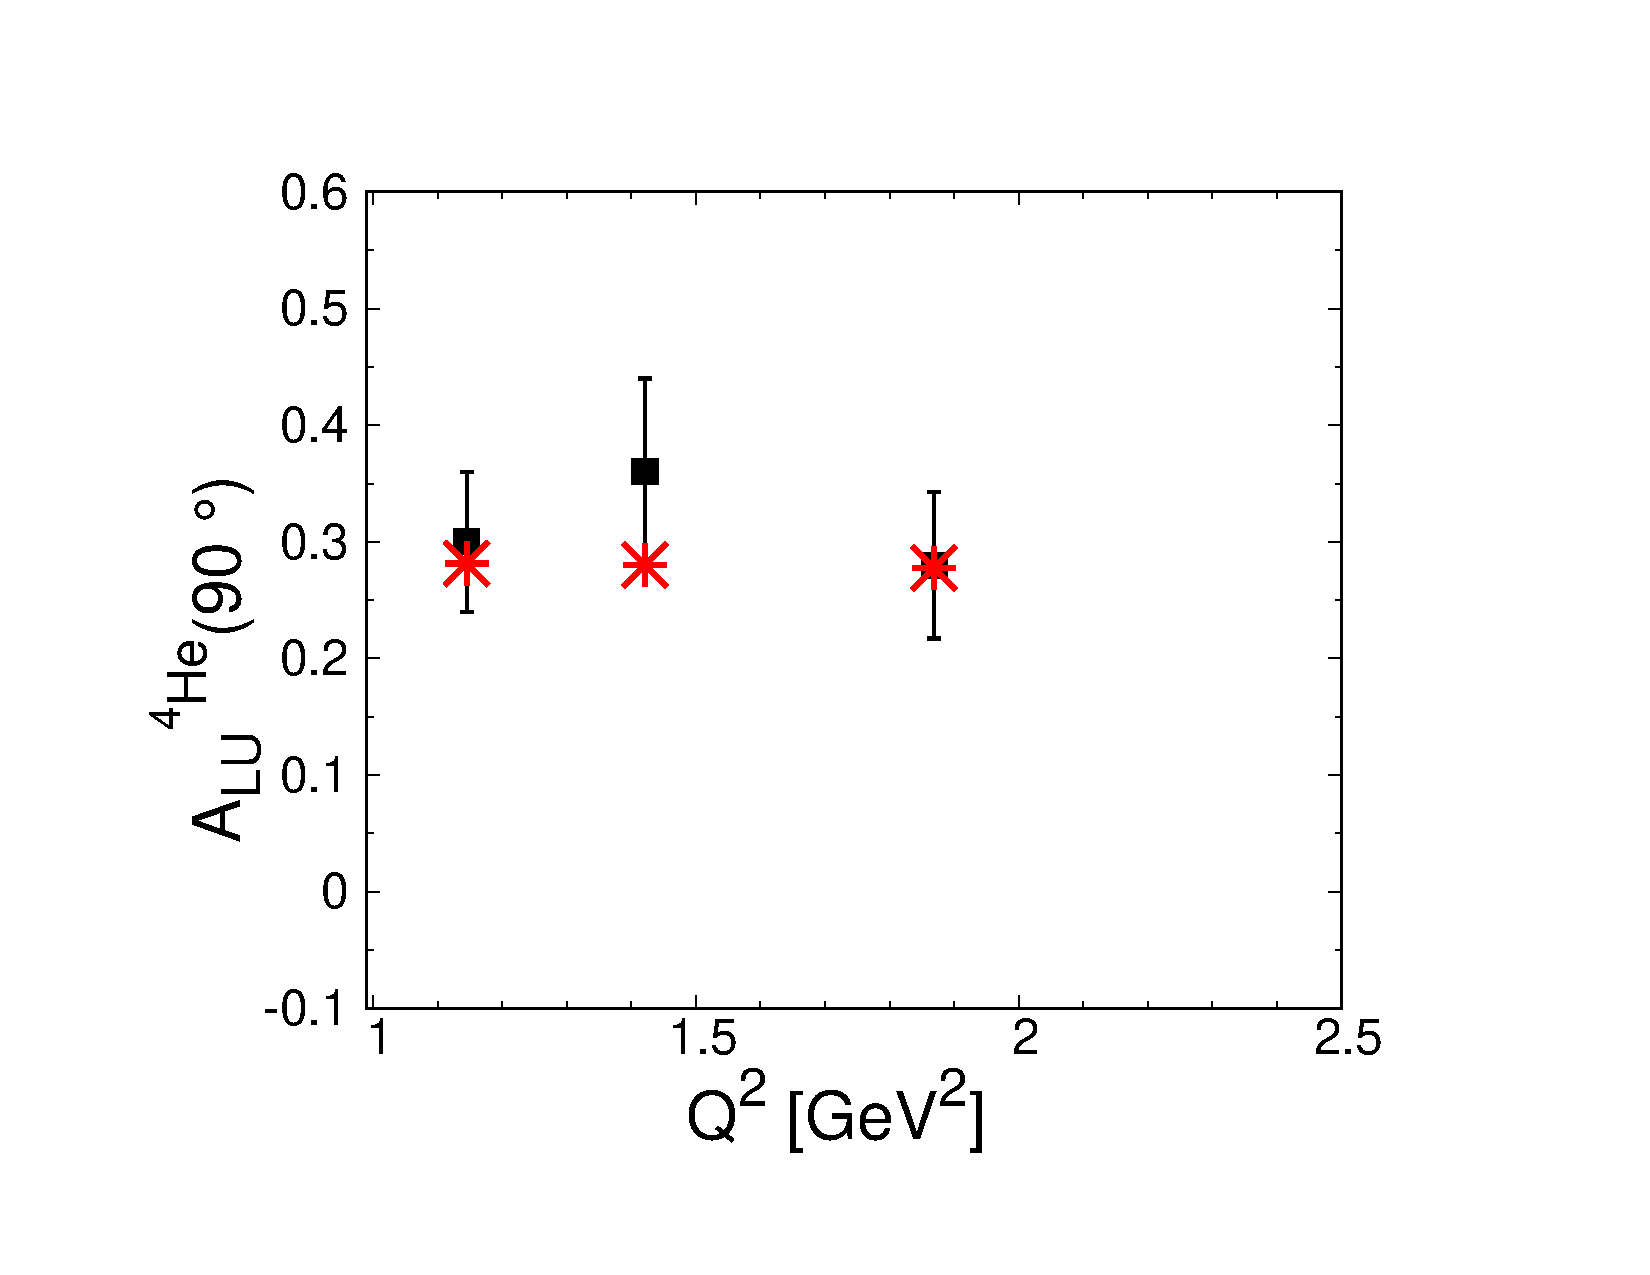
\includegraphics[scale=0.28]{plots/aluq2.pdf}
\vskip -1.cm
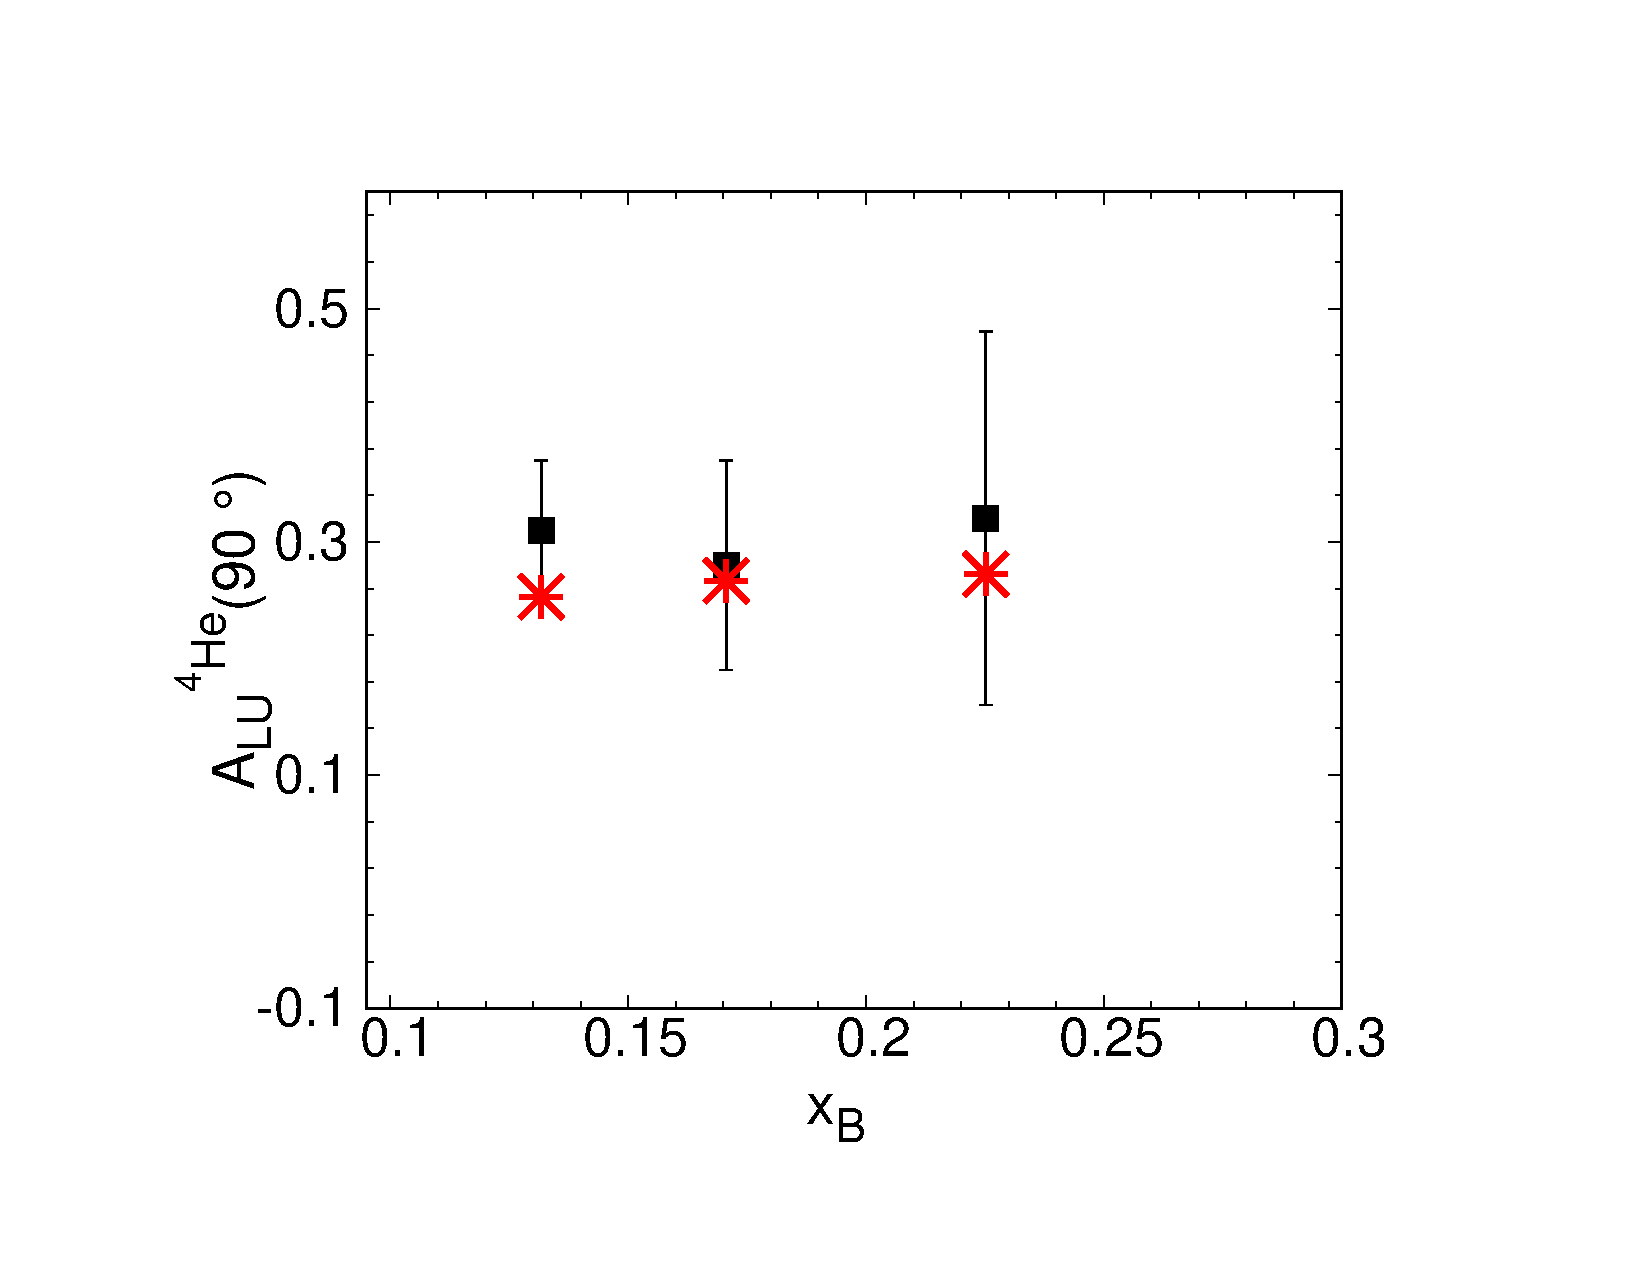
\includegraphics[scale=0.28]{plots/aluxb.pdf}
\vskip -1.cm
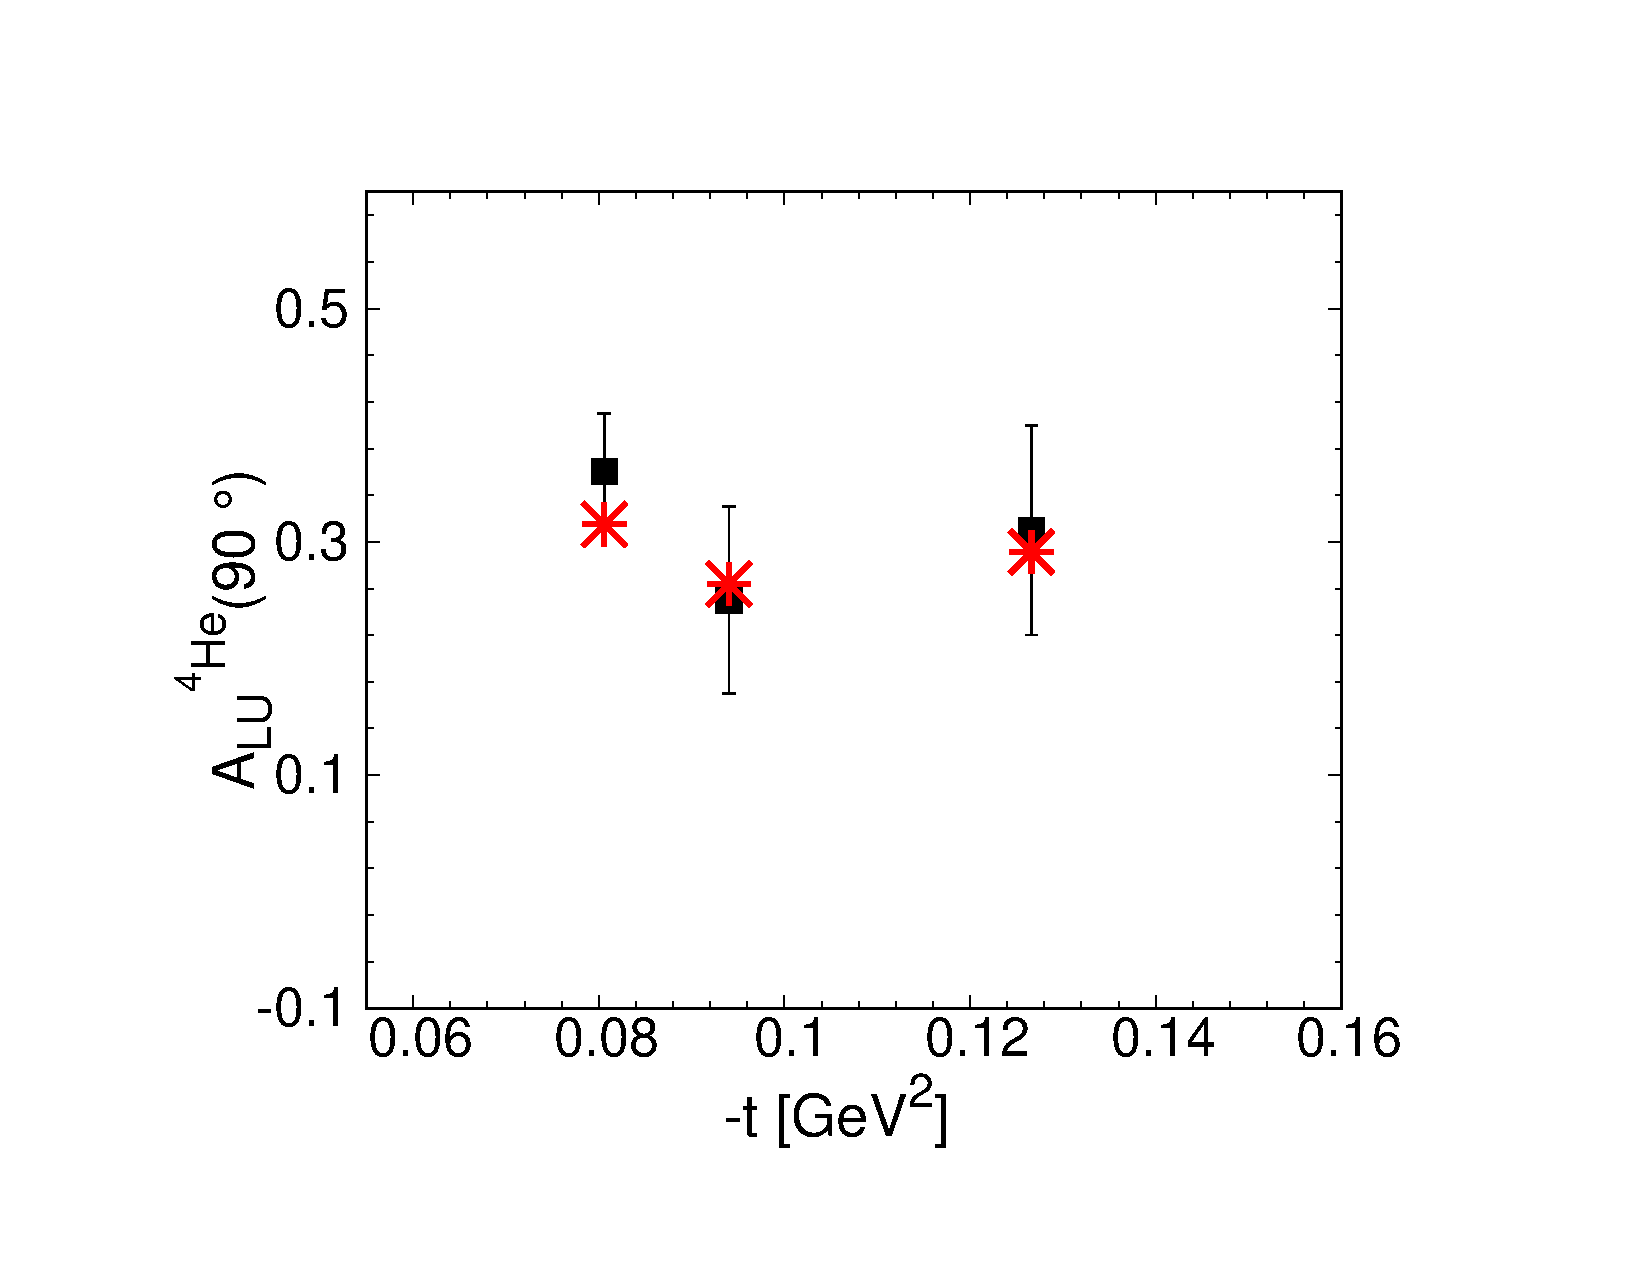
\includegraphics[scale=0.28]{plots/alut.pdf}
\vskip -.5cm
\caption{(Color online) $^4$He azimuthal beam-spin asymmetry $A_{LU}(\phi)$,
for $\phi = 90^o$: results of Ref. \cite{sara} (red stars) compared with data
(black squares)
\cite{Hattawy:2017woc}.
From top to bottom, the quantity is shown in the experimental
$Q^2$, $x_B$ and $t$ bins, respectively. 
}
\label{alu}
\end{figure}

The valence region at intermediate $Q^2$, investigated by 
JLab at 12 GeV, is crucial to access
the most discussed region of the EMC effect.
For light nuclei, such as $^2$H, $^3$He, $^4$He,
a realistic evaluation of conventional nuclear effects,
although sometimes challenging, is possible.
This would allow one to distinguish them
from exotic effects, which could be responsible for
the observed EMC behavior.
Without realistic benchmark calculations,  
interpreting experimental data cannot be conclusive.

%$^2$H is very interesting, both for its rich spin structure
%and for the the possible extraction of neutron information.
%$^4$He, being scalar and isoscalar, and a deeply bound 
%finite nucleus, is ideal to start with.
%In between these two targets, $^3$He provides an opportunity
%to study the $A$ dependence of nuclear effects, and
%it could give an easy access to neutron polarization properties,
%due to its specific spin structure.
%In addition, being isospin-$1/2$, it allows for the
%flavor dependence of nuclear effects could be studied, 
%in particular if parallel measurements 
%on $^3$H targets were possible \cite{Scopetta:2009sn}.

$^2$H is very interesting, both for its rich spin structure
and for the possibility of extracting free neutron information.
As a spin-one object, the deuteron admits a large number of GPDs,
as well as electromagnetic and gravitational form factors,
which encode more information than is available in the proton or neutron alone.
For instance, the deuteron appears to have two $D$-terms which encode
the distribution of shear and pressure, while the nucleon has one.
Understanding how forces are distributed in the deuteron
will give significant new insight into the role that QCD plays
in the nucleon-nucleon interaction. DVCS and DVMP on polarized deuterons
will allow much of this rich structure to be extracted.

$^4$He is the ideal deeply-bound nucleus to start with,
since it is scalar and isoscalar, and thus admits a simple
description in terms of its spin and flavor structure.
In between this and $^2$H, $^3$He provides an opportunity
to study the $A$ dependence of nuclear effects, and
it could give easy access to neutron polarization properties,
due to its specific spin structure.
In addition, being isospin-$1/2$, it allows for the
flavor dependence of nuclear effects could be studied, 
in particular if parallel measurements 
on $^3$H targets were possible \cite{Scopetta:2009sn}.

Due to very small cross sections,
especially in the coherent channel where the nucleus does not break-up,
the addressed measurements are very difficult.
Despite this, the first data for coherent DVCS off $^4$He,
collected at JLab, with the 6 GeV electron beam,
have been published \cite{Hattawy:2017woc}.
A new impressive program is on the way at JLab,
carried on by the ALERT collaboration 
\cite{Armstrong:2017wfw,Armstrong:2017zcm,Armstrong:2017zqr}.
Measurements for $^3$He and $^3$H
are not planned, but could be considered
for the upgrade of the ALERT project, at least in the unpolarized 
sector. Polarized measurements, which could
access neutron angular momentum information \cite{Rinaldi:2012pj,
Rinaldi:2012ft,Rinaldi:2014bba}, seem
very unlikely at JLab, due to the difficulty of arranging
a polarized target and a recoil detector very close to each other. 

From the theoretical point of view, a realistic calculation 
of conventional effects for
nuclear few-body systems corresponds to a plane wave impulse approximation 
(IA) analysis. This requires the evaluation of realistic non-diagonal spectral
functions for $^3$He and $^4$He.
For the first target, a complete analysis using the Argonne 18 (Av18)
nucleon-nucleon (NN) potential is available
\cite{Scopetta:2004kj,Scopetta:2009sn,Rinaldi:2012pj,
Rinaldi:2012ft,Rinaldi:2014bba}.
Nuclear GPDs are found to be sensitive to details of 
the used NN interaction.
A study with nuclear ingredients of the same quality
for $^4$He is still missing and should be performed, to update 
existing calculations \cite{Guzey:2003jh,Liuti:2005gi}. 
The evaluation of a realistic spectral functions of $^4$He,
using state-of-the-art NN potentials,
will require the wave function of a three-body scattering state, 
which is a really challenging problem.
Besides, in the incoherent channel of DVCS off $^2$H, $^3$He, $^4$He,
even the study of specific final state interactions will be necessary.

An encouraging approximate calculation has been recently
performed for coherent DVCS off $^4$He \cite{sara}, with the aim of
describing the CLAS data, as an intermediate
step towards a realistic evaluation.
A model of the nuclear non-diagonal spectral function, 
based on the momentum distribution
corresponding to the Av18 NN interaction
\cite{vivia}, has been used in the 
actual IA
calculation. Typical results
are found, in the proper limits, for the nuclear form factor
and for nuclear parton distributions.
Nuclear GPDs and
Compton form factors are evaluated using, as the nucleonic ingredient,
a well known GPD model \cite{gk}. 
As can be seen in Fig. \ref{alu}, a very good agreement 
is found with the data.  
One can conclude that 
a careful analysis of the reaction mechanism in terms of
basic conventional ingredients is successful and that
the present experimental accuracy does not require
the use of exotic arguments, such as dynamical off-shellness.
More refined nuclear calculations will be certainly necessary for 
the expected improved accuracy of the next generation of experiments 
at JLab, with the 12 GeV electron beam and high luminosity. 

Realistic calculations of $^2$H GPDs and Compton form factors using
state-of-the-art NN potentials are also available\cite{Cano:2003ju}.
Due to the breaking of Lorentz covariance through a Fock space truncation,
the extraction of gravitational form factors---including those describing
the distributions of mass, spin, pressure, and shear---is ambiguous.
It is possible to model $^2$H GPDs using
a simpler contact interaction while maintaining covariance, and thus
make unambiguous predictions for GFFs and the stress-energy tensor.
This has the shortcoming of using a less realistic interaction,
and is limited to a domain where $t$ is very small. Manifestly covariant
calculations of nuclear structure with more realistic NN interactions
are sorely needed for GPD calculations, since GPDs are the only experimental
avenue through which GFFs can be accessed.
  
While JLab will provide important information
in the valence region, the extension to lower
$x$ values will be possible only at the EIC \cite{Accardi:2012qut}. 
Great opportunities at the EIC are also those related to the possibility
of easily using $^3$H beams, or polarized trinucleon beams and 
recoil detectors at the same time, to access, for example, 
the neutron polarized structure and the flavor dependence 
of nuclear effects.





